\section{Event-based Systems}

\subsection{Ereignisse (Events)}

Reaktive Systeme reagieren auf (oft externe) Ereignisse (z.B. Digitale Inputs, Timer, Buttonclicks, etc.). Solche \textbf{Ereignisse sind per 
Definition asynchron und treten somit zu einem beliebigen Zeitpunkt auf.} 
Die Ereignisse können jedoch \textbf{synchron oder asynchron} umgesetzt werden.


\subsection{Synchrone Umsetzung von Ereignissen}

Ein '\textbf{normales' Programm} ist immer \textbf{synchron}. (Programm gibt vor, was wann ausgeführt wird.)

\subsubsection{Polling}

\begin{itemize}
    \item Programm fragt periodisch oder dauernd ab, ob irgendein Ereignis eingetreten ist
    \item Maximale Reaktionszeit wird durch Abfrageperiode und Anzahl Abfragen definiert (Looptime bei SPS)
    \item[+] Sehr einfach zu implementieren
    \item[-] Leerabfragen (Abfragen, bei welchen nichts eingetreten ist) können durch periodisches Abfragen (mittels Timer) reduziert, 
        aber nicht vermieden werden
\end{itemize}


\subsection{Asynchrone Umsetzung von Ereignissen}

Ziel der asynchronen Verarbeitung von Events ist es, dass die Prozessorzeit \textbf{genau dann und nur dann} beansprucht wird, wenn ein 
Ereignis eingetreten ist. \textrightarrow\ Interrupts


\subsection{Interrupt-Verarbeitung}

\begin{enumerate}
    \item I/O-Element generiert einen Interrupt Request
    \item Die CPU unterbricht das laufende Programm
    \item \textbf{Die Interrupts werden disabled (ausgeschaltet)}
    \item Das I/O-Element wird informiert, dieses deaktiviert den Interrupt Request
    \item Die Interrupt Service Routine (ISR) wird ausgeführt
    \item \textbf{Die Interrupts werden wieder enabled (eingeschaltet)}
    \item Die CPU führt das Programm an der unterbrochenen Stelle weiter
\end{enumerate}


\para{Sprungadresse nach Interrupt-Auslösung (ISR)}

\begin{outline}
    \1 \textbf{Non-vectored Interrupt (zentral)}
        \2 Alle Interrupts verzweigen zu einer \textbf{gemeinsamen Adresse}. Dort wird die Ursache bestimmt und zu einer
            spezifischen Behandlungsroutine verzweigt.
        \2[+] Nur eine zentrale Routine für die Behandlung notwendig
        \2[-] Information über die Ursache ist beim Eintreten bereits bekannt. Dann
                verzweigt man in die zentrale Routine, d.h. diese Information ist dann verloren. In der Routine muss diese
                Information wieder ermittelt werden.
    \1 \textbf{Vectored Interrupt (spezifisch)}
        \2 In einer Tabelle (\textbf{Interruptvektortabelle}, IVT) wird gespeichert, wohin bei welchem Interruptvektor
            verzweigt werden muss. \\
            \textrightarrow\ zu bevorzugende Methode!
\end{outline}


\subsection{Interruptvektortabelle (IVT)}

Für jeden Vektor muss eingetragen werden, welches die \textbf{Anfangsadresse} der Interrupt Service Routine
(ISR) ist, d.h. die \textbf{IVT ist nichts anderes als eine Tabelle (Array) von Funktionspointern.}

\vspace{0.1cm}

\textrightarrow\ Dieses Konzept kommt bei \textbf{allen asynchronen Mechanismen} zur Anwendung


\subsection{Model View Controller (MVC) aka Observer Pattern}

Ausgangslage: Daten (model) und verschiedene Darstellungsformen (views) der Daten (z.B. Balkendiagramm, Kuchendiagramm, Tabelle, etc.) \\
\textbf{\textrightarrow\ Die views sollen unbedingt vom model getrennt werden!}

\vspace{0.2cm}

Wie kann nun erreicht werden, dass bei \textbf{jeder Änderung} der Daten (model) alle Darstellungen aktualisiert werden? 
\textrightarrow\ Callback-Funktionen!


\subsection{Callback-Funktionen}

\begin{itemize}
    \item[+] Views werden \textbf{asynchron} genau informiert, wenn sich etwas im \textbf{model geändert} hat
    \item[+] An und für sich sind alle registrierten Funktionen nichts anderes als \textbf{Eventhandler eines bestimmten Events}
        \textrightarrow\ Darstellung (Definition der registrierten Funktionen) sauber von den Daten (model) \textbf{entkoppelt} 
\end{itemize}


\subsubsection{Callback-Funktionen in C}

Beim MVC gilt:

\vspace{0.1cm}

\begin{itemize}
    \item model wirkt als server
    \item views sind clients
\end{itemize}


\para{Event registieren (attach)}

\begin{outline}
    \1 Jeder client meldet beim server an, welche Ereignisse ihn interessieren
        \2 Anmeldung erfolgt über eine Funktion, welche der service anbietet
        \lstinputlisting[aboveskip=1mm, linewidth=\linewidth, morekeywords={[3], e, f}, firstnumber=1, firstline=1, lastline=3]{snippets/ebs_callback.c}
    \1 Der server trägt diesen \textbf{Funktionspointer} \mylstbox{f} in eine Tabelle ein und ruft \textbf{beim Eintreten des Ereignisses alle
        registrierten Funktionen} der Reihe nach je über den eingetragenen Funktionspointer auf
\end{outline}


\para{Event austragen (detach)}

\begin{outline}
    \1 Ein client kann sein Interesse an einem Ereignis beim Server auch wieder austragen
        \2 Der Server löscht dann den entsprechenden Eintrag (\textbf{Funktionspointer} \mylstbox{f}) wieder aus der Tabelle
        \lstinputlisting[aboveskip=1mm, linewidth=\linewidth, morekeywords={[3], e, f}, firstnumber=1, firstline=5, lastline=7]{snippets/ebs_callback.c}
\end{outline}


\subsection{Umsetzung der Callback-Funktionen in C (serverseitig)} 

\begin{outline}
    \1 Funktionspointer \mylstbox{foo_cbFunction} zu Callback-Funktionen definieren
        \lstinputlisting[aboveskip=1mm, linewidth=\linewidth, firstnumber=1, firstline=9, lastline=10]{snippets/ebs_callback.c}
    \1 Tabelle von Funktionspointern für jeden Event definieren und mit \textbf{Nullpointern initialisieren}
        \lstinputlisting[aboveskip=1mm, linewidth=\linewidth, morekeywords={[3], evNum, evClient}, firstnumber=1, firstline=12, lastline=13]{snippets/ebs_callback.c}
    \1 Aufruf der registrierten Clientfunktionen beim Eintreten des Events
        \lstinputlisting[aboveskip=1mm, linewidth=\linewidth, morekeywords={[3], evNum, i, evClient, client, arg}, firstnumber=1, firstline=15, lastline=24]{snippets/ebs_callback.c}
\end{outline}


\para{Mitteilung eines Events}

\vspace{0.1cm}

\begin{minipage}[t]{0.4\columnwidth}
    \raggedright
    Sobald (\textbf{asynchron}) ein Event eingetreten ist, kann dieser dem Server mit der Funktion
    \mylstbox[morekeywords={[3], e}]{void  foo_signalEvent(foo_Event e);} mitgeteilt werden.
\end{minipage}
\hfill
\begin{minipage}[t]{0.56\columnwidth}
    % CHECK: If there will be a full code example of callback functions, outcomment the following snippet
    \lstinputlisting[aboveskip=1mm, linewidth=\linewidth, morekeywords={[3], e, ev1Num, ev2Num, ev1Client, ev2Vlient}, firstnumber=1, firstline=26, lastline=42]{snippets/ebs_callback.c}
\end{minipage}


% Sobald (\textbf{asynchron}) ein Event eingetreten ist, kann dieser dem Server mit der Funktion
% \mylstbox[morekeywords={[3], e}]{void  foo_signalEvent(foo_Event e);} mitgeteilt werden.

% % CHECK: If there will be a full code example of callback functions, outcomment the following snippet
% \lstinputlisting[aboveskip=1mm, linewidth=\linewidth, morekeywords={[3], e, ev1Num, ev2Num, ev1Client, ev2Vlient}, firstnumber=1, firstline=26, lastline=42]{snippets/ebs_callback.c}


\subsection{Observer Pattern}

\subsubsection{Klassendiagramm (abstrakte Observer Basisklasse)}

\begin{center}
    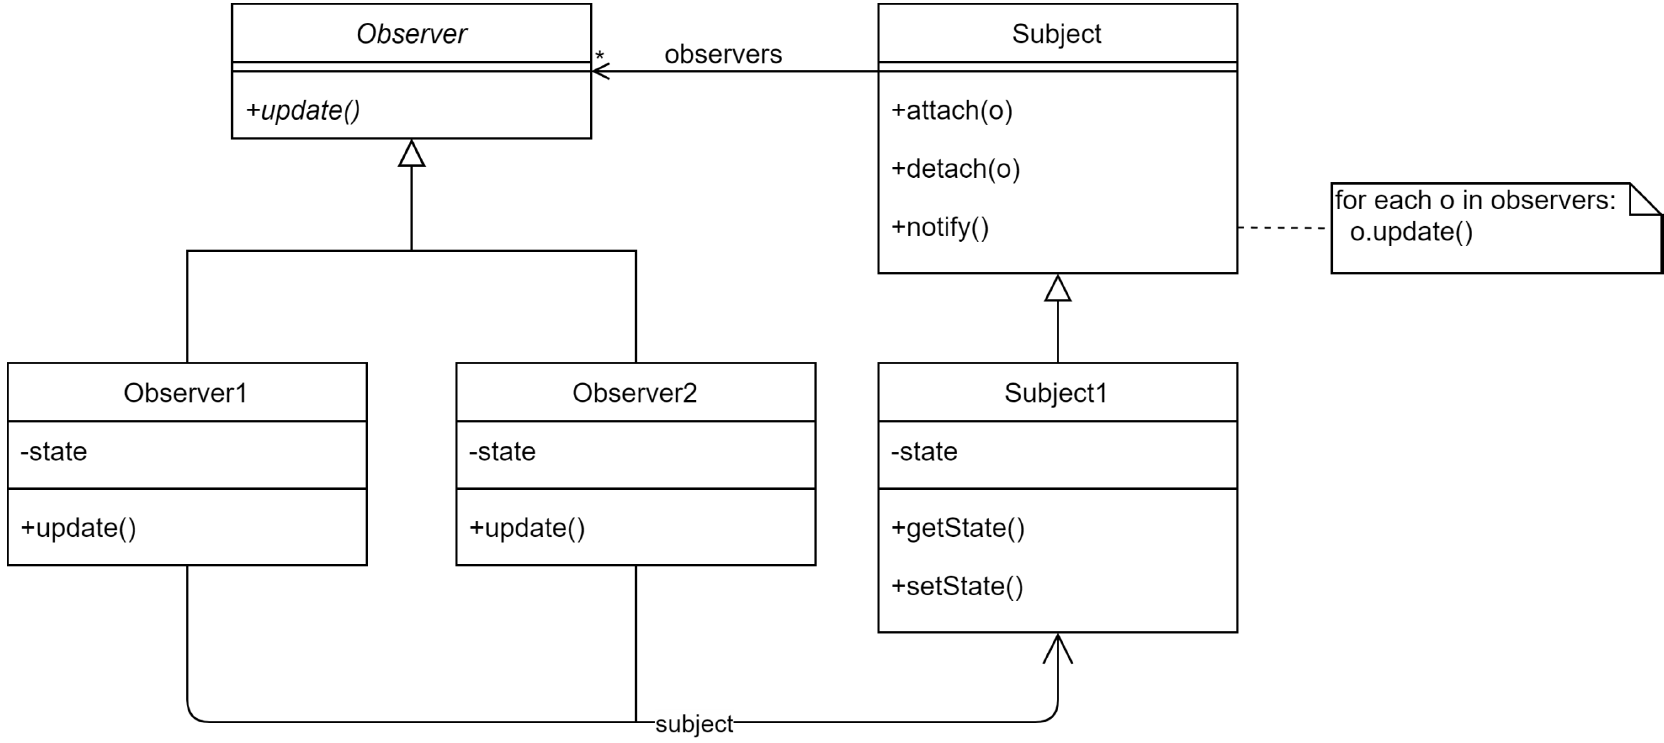
\includegraphics[width=0.8\columnwidth]{images/ebs_observer_pattern_klassendiagramm.png}
\end{center}


\subsubsection{Implementation in C++}

%TODO: write some stuff about how to implmenent that stuff
% slide 20 + eigene Erkenntnisse / Gedanken

\begin{outline}
    \1 \textbf{Observer-Klasse (abstrakte Basisklasse)}

    \1 \textbf{Observer-Subklassen}

    \1 \textbf{Subjekt Klasse}

    \1 \textbf{Subjekt1 Subklasse}
\end{outline}


\example{Observer Pattern in C++}

%TODO: code snippets